\documentclass[sigconf,anonymous]{acmart}

\usepackage{booktabs} % For formal tables

% XS: add command
\newcommand{\norm}[1]{|\!|#1|\!|}
\newcommand{\N}{{\mathbb{N}}}
\newcommand{\R}{{\mathbb{R}}}
\newcommand{\W}{{\mathcal{W}}}



\usepackage{color}
\renewcommand{\r}[1]{{{{\color{red}#1}}}}
\renewcommand{\b}[1]{{{{\color{blue}#1}}}}


% Copyright
%\setcopyright{none}
%\setcopyright{acmcopyright}
%\setcopyright{acmlicensed}
\setcopyright{rightsretained}
%\setcopyright{usgov}
%\setcopyright{usgovmixed}
%\setcopyright{cagov}
%\setcopyright{cagovmixed}


% DOI
\acmDOI{XXXX/XXXX}

% ISBN
\acmISBN{XXX-XXXX-XX-XXX/XX/XX}

%Conference
\acmConference[HSCC'19]{ACM International Conference on 
Hybrid Systems: Computation and Control}{April 2019}{Montreal, Canada}
\acmYear{2019}
\copyrightyear{2019}


%\acmArticle{X}
%\acmPrice{XX}

% These commands are optional
%\acmBooktitle{Transactions of the ACM Woodstock conference}
%\editor{Jennifer B. Sartor}
%\editor{Theo D'Hondt}
%\editor{Wolfgang De Meuter}

\settopmatter{printacmref=false}



\begin{document}
\title{System-Level Verification of Neural Network Controlled Autonomous Systems}

%\titlenote{Produces the permission block, and copyright information}
%\subtitle{Extended Abstract}
%\subtitlenote{The full version of the author's guide is available as
%  \texttt{acmart.pdf} document}

%
%\author{Ben Trovato}
%\authornote{Dr.~Trovato insisted his name be first.}
%\orcid{1234-5678-9012}
%\affiliation{%
%  \institution{Institute for Clarity in Documentation}
%  \streetaddress{P.O. Box 1212}
%  \city{Dublin}
%  \state{Ohio}
%  \postcode{43017-6221}
%}
%\email{trovato@corporation.com}
%
%\author{G.K.M. Tobin}
%\authornote{The secretary disavows any knowledge of this author's actions.}
%\affiliation{%
%  \institution{Institute for Clarity in Documentation}
%  \streetaddress{P.O. Box 1212}
%  \city{Dublin}
%  \state{Ohio}
%  \postcode{43017-6221}
%}
%\email{webmaster@marysville-ohio.com}
%
%\author{Lars Th{\o}rv{\"a}ld}
%\authornote{This author is the
%  one who did all the really hard work.}
%\affiliation{%
%  \institution{The Th{\o}rv{\"a}ld Group}
%  \streetaddress{1 Th{\o}rv{\"a}ld Circle}
%  \city{Hekla}
%  \country{Iceland}}
%\email{larst@affiliation.org}
%
%\author{Valerie B\'eranger}
%\affiliation{%
%  \institution{Inria Paris-Rocquencourt}
%  \city{Rocquencourt}
%  \country{France}
%}
%\author{Aparna Patel}
%\affiliation{%
% \institution{Rajiv Gandhi University}
% \streetaddress{Rono-Hills}
% \city{Doimukh}
% \state{Arunachal Pradesh}
% \country{India}}
%\author{Huifen Chan}
%\affiliation{%
%  \institution{Tsinghua University}
%  \streetaddress{30 Shuangqing Rd}
%  \city{Haidian Qu}
%  \state{Beijing Shi}
%  \country{China}
%}
%
%\author{Charles Palmer}
%\affiliation{%
%  \institution{Palmer Research Laboratories}
%  \streetaddress{8600 Datapoint Drive}
%  \city{San Antonio}
%  \state{Texas}
%  \postcode{78229}}
%\email{cpalmer@prl.com}
%
%\author{John Smith}
%\affiliation{\institution{The Th{\o}rv{\"a}ld Group}}
%\email{jsmith@affiliation.org}
%
%\author{Julius P.~Kumquat}
%\affiliation{\institution{The Kumquat Consortium}}
%\email{jpkumquat@consortium.net}
%
%% The default list of authors is too long for headers.
%\renewcommand{\shortauthors}{B. Trovato et al.}


\begin{abstract}
In this paper, we consider the formal verification problem of an autonomous robot equipped with a LiDAR scanner and a Neural Network (NN) that processes the LiDAR images to produce control actions. Given a workspace that is characterized by a set of obstacles and a set of regions of interest, where both the obstacles and the regions are polyhedra, we show that the LiDAR imaging function (that maps the robot position to the LiDAR image) is a piecewise \r{affine} function. Based on this observation, we develop a \r{polynomial}-time algorithm that partitions the workspace into regions such that the LiDAR imaging is \r{affine}. Given this workspace partitioning, a discrete-time and linear dynamics of the robot, and a pre-trained NN controller with Rectified Linear Unit (ReLU) nonlinearity, our objective is to compute a finite transition abstraction of the NN-controlled system. Motivated by the NP-hardness of analyzing neural networks with ReLU nonlinearities, we develop a Satisfiability Modulo Convex (SMC) Programming algorithm that utilizes a Boolean satisfiability solver and a convex programming solver and decomposes the problem into smaller subproblems. At each iteration, the  Boolean satisfiability solver searches for a candidate assignment for the different ReLU phases while completely abstracting the robot dynamics. Convex programming is then used to check the feasibility of the proposed ReLU phases against the dynamic and imagining constraints, or generate succinct explanations for their infeasibility to reduce the search space. 
%This process needs to be executed while taking into considerations each combination of regions in the partitioned workspace.  To harness the exponential growth due to the large number of partitioned regions, our framework utilizes an abstraction refinement process in which coarse abstractions based on a smaller number of laser beams are first considered and the refined if deemed necessary by the SMC-based procedure. 
Finally, given the computed finite transition abstraction along with a system-level property $\varphi$ captured by Linear-Temporal Logic (LTL), our framework can verify if the NN-controlled system satisfies $\varphi$. Numerical results show the effectiveness of our framework in proving the safety of a NN-controlled robot with \r{XX} continuous states and a neural network consisting of \r{XX} neurons.
\end{abstract}

%
% The code below should be generated by the tool at
% http://dl.acm.org/ccs.cfm
% Please copy and paste the code instead of the example below.
%
%\begin{CCSXML}
%<ccs2012>
% <concept>
%  <concept_id>10010520.10010553.10010562</concept_id>
%  <concept_desc>Computer systems organization~Embedded systems</concept_desc>
%  <concept_significance>500</concept_significance>
% </concept>
% <concept>
%  <concept_id>10010520.10010575.10010755</concept_id>
%  <concept_desc>Computer systems organization~Redundancy</concept_desc>
%  <concept_significance>300</concept_significance>
% </concept>
% <concept>
%  <concept_id>10010520.10010553.10010554</concept_id>
%  <concept_desc>Computer systems organization~Robotics</concept_desc>
%  <concept_significance>100</concept_significance>
% </concept>
% <concept>
%  <concept_id>10003033.10003083.10003095</concept_id>
%  <concept_desc>Networks~Network reliability</concept_desc>
%  <concept_significance>100</concept_significance>
% </concept>
%</ccs2012>
%\end{CCSXML}
%
%\ccsdesc[500]{Computer systems organization~Embedded systems}
%\ccsdesc[300]{Computer systems organization~Redundancy}
%\ccsdesc{Computer systems organization~Robotics}
%\ccsdesc[100]{Networks~Network reliability}


\keywords{Formal verification, Machine Learning, Satisfiability Solvers}


\maketitle

%\section{Introduction}

The \textit{proceedings} are the records of a conference.\footnote{This
  is a footnote}  ACM seeks
to give these conference by-products a uniform, high-quality
appearance.  To do this, ACM has some rigid requirements for the
format of the proceedings documents: there is a specified format
(balanced double columns), a specified set of fonts (Arial or
Helvetica and Times Roman) in certain specified sizes, a specified
live area, centered on the page, specified size of margins, specified
column width and gutter size.

\section{The Body of The Paper}
Typically, the body of a paper is organized into a hierarchical
structure, with numbered or unnumbered headings for sections,
subsections, sub-subsections, and even smaller sections.  The command
\texttt{{\char'134}section} that precedes this paragraph is part of
such a hierarchy.\footnote{This is a footnote.} \LaTeX\ handles the
numbering and placement of these headings for you, when you use the
appropriate heading commands around the titles of the headings.  If
you want a sub-subsection or smaller part to be unnumbered in your
output, simply append an asterisk to the command name.  Examples of
both numbered and unnumbered headings will appear throughout the
balance of this sample document.

Because the entire article is contained in the \textbf{document}
environment, you can indicate the start of a new paragraph with a
blank line in your input file; that is why this sentence forms a
separate paragraph.

\subsection{Type Changes and {\itshape Special} Characters}

We have already seen several typeface changes in this sample.  You can
indicate italicized words or phrases in your text with the command
\texttt{{\char'134}textit}; emboldening with the command
\texttt{{\char'134}textbf} and typewriter-style (for instance, for
computer code) with \texttt{{\char'134}texttt}.  But remember, you do
not have to indicate typestyle changes when such changes are part of
the \textit{structural} elements of your article; for instance, the
heading of this subsection will be in a sans serif\footnote{Another
  footnote here.  Let's make this a rather long one to see how it
  looks.} typeface, but that is handled by the document class file.
Take care with the use of\footnote{Another footnote.}  the
curly braces in typeface changes; they mark the beginning and end of
the text that is to be in the different typeface.

You can use whatever symbols, accented characters, or non-English
characters you need anywhere in your document; you can find a complete
list of what is available in the \textit{\LaTeX\ User's Guide}
\cite{Lamport:LaTeX}.

\subsection{Math Equations}
You may want to display math equations in three distinct styles:
inline, numbered or non-numbered display.  Each of
the three are discussed in the next sections.

\subsubsection{Inline (In-text) Equations}
A formula that appears in the running text is called an
inline or in-text formula.  It is produced by the
\textbf{math} environment, which can be
invoked with the usual \texttt{{\char'134}begin\,\ldots{\char'134}end}
construction or with the short form \texttt{\$\,\ldots\$}. You
can use any of the symbols and structures,
from $\alpha$ to $\omega$, available in
\LaTeX~\cite{Lamport:LaTeX}; this section will simply show a
few examples of in-text equations in context. Notice how
this equation:
\begin{math}
  \lim_{n\rightarrow \infty}x=0
\end{math},
set here in in-line math style, looks slightly different when
set in display style.  (See next section).

\subsubsection{Display Equations}
A numbered display equation---one set off by vertical space from the
text and centered horizontally---is produced by the \textbf{equation}
environment. An unnumbered display equation is produced by the
\textbf{displaymath} environment.

Again, in either environment, you can use any of the symbols
and structures available in \LaTeX\@; this section will just
give a couple of examples of display equations in context.
First, consider the equation, shown as an inline equation above:
\begin{equation}
  \lim_{n\rightarrow \infty}x=0
\end{equation}
Notice how it is formatted somewhat differently in
the \textbf{displaymath}
environment.  Now, we'll enter an unnumbered equation:
\begin{displaymath}
  \sum_{i=0}^{\infty} x + 1
\end{displaymath}
and follow it with another numbered equation:
\begin{equation}
  \sum_{i=0}^{\infty}x_i=\int_{0}^{\pi+2} f
\end{equation}
just to demonstrate \LaTeX's able handling of numbering.

\subsection{Citations}
Citations to articles~\cite{bowman:reasoning,
clark:pct, braams:babel, herlihy:methodology},
conference proceedings~\cite{clark:pct} or maybe
books \cite{Lamport:LaTeX, salas:calculus} listed
in the Bibliography section of your
article will occur throughout the text of your article.
You should use BibTeX to automatically produce this bibliography;
you simply need to insert one of several citation commands with
a key of the item cited in the proper location in
the \texttt{.tex} file~\cite{Lamport:LaTeX}.
The key is a short reference you invent to uniquely
identify each work; in this sample document, the key is
the first author's surname and a
word from the title.  This identifying key is included
with each item in the \texttt{.bib} file for your article.

The details of the construction of the \texttt{.bib} file
are beyond the scope of this sample document, but more
information can be found in the \textit{Author's Guide},
and exhaustive details in the \textit{\LaTeX\ User's
Guide} by Lamport~\shortcite{Lamport:LaTeX}.

This article shows only the plainest form
of the citation command, using \texttt{{\char'134}cite}.

Some examples.  A paginated journal article \cite{Abril07}, an enumerated
journal article \cite{Cohen07}, a reference to an entire issue \cite{JCohen96},
a monograph (whole book) \cite{Kosiur01}, a monograph/whole book in a series (see 2a in spec. document)
\cite{Harel79}, a divisible-book such as an anthology or compilation \cite{Editor00}
followed by the same example, however we only output the series if the volume number is given
\cite{Editor00a} (so Editor00a's series should NOT be present since it has no vol. no.),
a chapter in a divisible book \cite{Spector90}, a chapter in a divisible book
in a series \cite{Douglass98}, a multi-volume work as book \cite{Knuth97},
an article in a proceedings (of a conference, symposium, workshop for example)
(paginated proceedings article) \cite{Andler79}, a proceedings article
with all possible elements \cite{Smith10}, an example of an enumerated
proceedings article \cite{VanGundy07},
an informally published work \cite{Harel78}, a doctoral dissertation \cite{Clarkson85},
a master's thesis: \cite{anisi03}, an online document / world wide web
resource \cite{Thornburg01, Ablamowicz07, Poker06}, a video game (Case 1) \cite{Obama08} and (Case 2) \cite{Novak03}
and \cite{Lee05} and (Case 3) a patent \cite{JoeScientist001},
work accepted for publication \cite{rous08}, 'YYYYb'-test for prolific author
\cite{SaeediMEJ10} and \cite{SaeediJETC10}. Other cites might contain
'duplicate' DOI and URLs (some SIAM articles) \cite{Kirschmer:2010:AEI:1958016.1958018}.
Boris / Barbara Beeton: multi-volume works as books
\cite{MR781536} and \cite{MR781537}.

A couple of citations with DOIs: \cite{2004:ITE:1009386.1010128,
  Kirschmer:2010:AEI:1958016.1958018}.

Online citations: \cite{TUGInstmem, Thornburg01, CTANacmart}.


\subsection{Tables}
Because tables cannot be split across pages, the best
placement for them is typically the top of the page
nearest their initial cite.  To
ensure this proper ``floating'' placement of tables, use the
environment \textbf{table} to enclose the table's contents and
the table caption.  The contents of the table itself must go
in the \textbf{tabular} environment, to
be aligned properly in rows and columns, with the desired
horizontal and vertical rules.  Again, detailed instructions
on \textbf{tabular} material
are found in the \textit{\LaTeX\ User's Guide}.

Immediately following this sentence is the point at which
Table~\ref{tab:freq} is included in the input file; compare the
placement of the table here with the table in the printed
output of this document.

\begin{table}
  \caption{Frequency of Special Characters}
  \label{tab:freq}
  \begin{tabular}{ccl}
    \toprule
    Non-English or Math&Frequency&Comments\\
    \midrule
    \O & 1 in 1,000& For Swedish names\\
    $\pi$ & 1 in 5& Common in math\\
    \$ & 4 in 5 & Used in business\\
    $\Psi^2_1$ & 1 in 40,000& Unexplained usage\\
  \bottomrule
\end{tabular}
\end{table}

To set a wider table, which takes up the whole width of the page's
live area, use the environment \textbf{table*} to enclose the table's
contents and the table caption.  As with a single-column table, this
wide table will ``float'' to a location deemed more desirable.
Immediately following this sentence is the point at which
Table~\ref{tab:commands} is included in the input file; again, it is
instructive to compare the placement of the table here with the table
in the printed output of this document.


\begin{table*}
  \caption{Some Typical Commands}
  \label{tab:commands}
  \begin{tabular}{ccl}
    \toprule
    Command &A Number & Comments\\
    \midrule
    \texttt{{\char'134}author} & 100& Author \\
    \texttt{{\char'134}table}& 300 & For tables\\
    \texttt{{\char'134}table*}& 400& For wider tables\\
    \bottomrule
  \end{tabular}
\end{table*}
% end the environment with {table*}, NOTE not {table}!

It is strongly recommended to use the package booktabs~\cite{Fear05}
and follow its main principles of typography with respect to tables:
\begin{enumerate}
\item Never, ever use vertical rules.
\item Never use double rules.
\end{enumerate}
It is also a good idea not to overuse horizontal rules.


\subsection{Figures}

Like tables, figures cannot be split across pages; the best placement
for them is typically the top or the bottom of the page nearest their
initial cite.  To ensure this proper ``floating'' placement of
figures, use the environment \textbf{figure} to enclose the figure and
its caption.

This sample document contains examples of \texttt{.eps} files to be
displayable with \LaTeX.  If you work with pdf\LaTeX, use files in the
\texttt{.pdf} format.  Note that most modern \TeX\ systems will convert
\texttt{.eps} to \texttt{.pdf} for you on the fly.  More details on
each of these are found in the \textit{Author's Guide}.

\begin{figure}
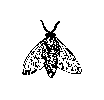
\includegraphics{figures/fly}
\caption{A sample black and white graphic.}
\end{figure}

\begin{figure}
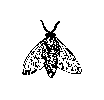
\includegraphics[height=1in, width=1in]{figures/fly}
\caption{A sample black and white graphic
that has been resized with the \texttt{includegraphics} command.}
\end{figure}


As was the case with tables, you may want a figure that spans two
columns.  To do this, and still to ensure proper ``floating''
placement of tables, use the environment \textbf{figure*} to enclose
the figure and its caption.  And don't forget to end the environment
with \textbf{figure*}, not \textbf{figure}!

\begin{figure*}
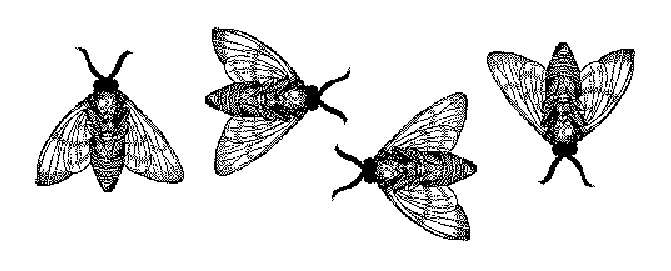
\includegraphics{figures/flies}
\caption{A sample black and white graphic
that needs to span two columns of text.}
\end{figure*}


\begin{figure}
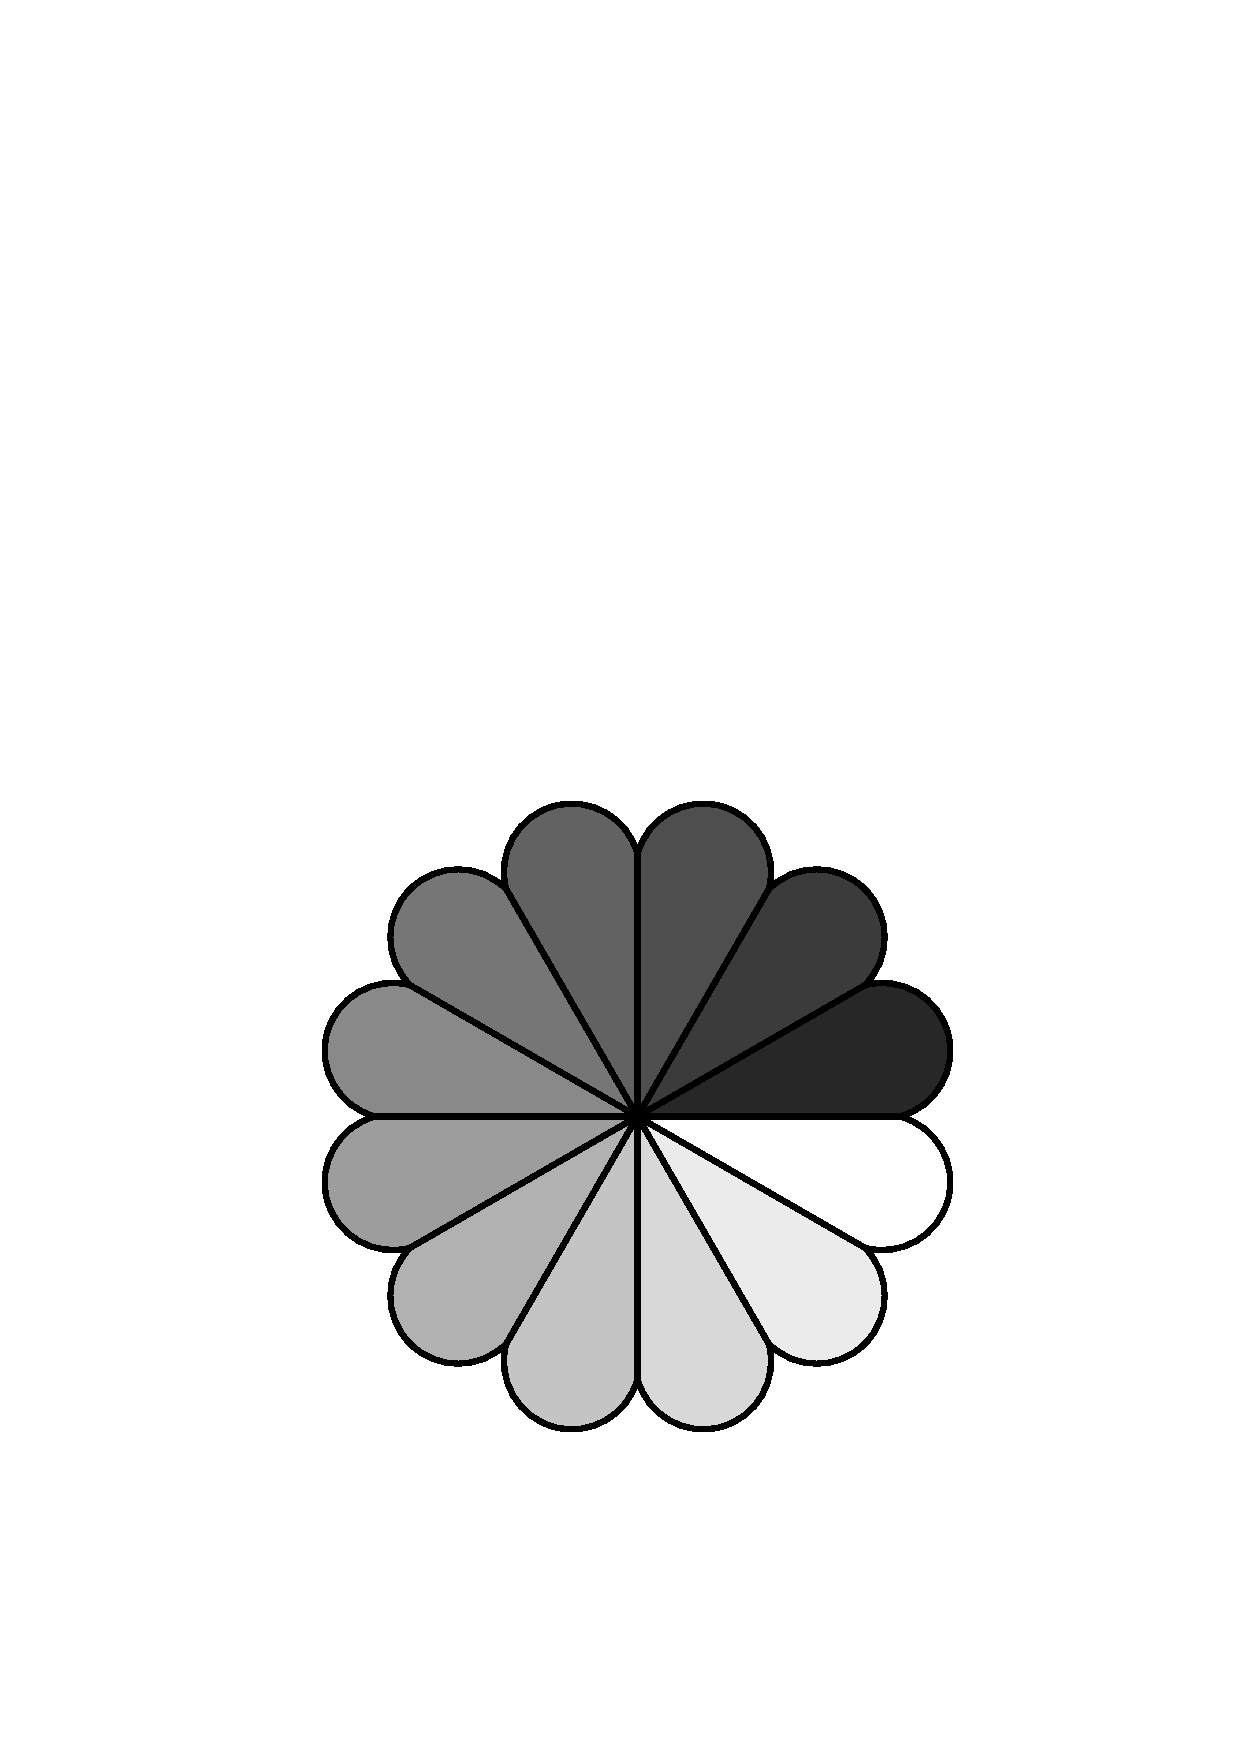
\includegraphics[height=1in, width=1in]{figures/rosette}
\caption{A sample black and white graphic that has
been resized with the \texttt{includegraphics} command.}
\end{figure}

\subsection{Theorem-like Constructs}

Other common constructs that may occur in your article are the forms
for logical constructs like theorems, axioms, corollaries and proofs.
ACM uses two types of these constructs:  theorem-like and
definition-like.

Here is a theorem:
\begin{theorem}
  Let $f$ be continuous on $[a,b]$.  If $G$ is
  an antiderivative for $f$ on $[a,b]$, then
  \begin{displaymath}
    \int^b_af(t)\,dt = G(b) - G(a).
  \end{displaymath}
\end{theorem}

Here is a definition:
\begin{definition}
  If $z$ is irrational, then by $e^z$ we mean the
  unique number that has
  logarithm $z$:
  \begin{displaymath}
    \log e^z = z.
  \end{displaymath}
\end{definition}

The pre-defined theorem-like constructs are \textbf{theorem},
\textbf{conjecture}, \textbf{proposition}, \textbf{lemma} and
\textbf{corollary}.  The pre-defined de\-fi\-ni\-ti\-on-like constructs are
\textbf{example} and \textbf{definition}.  You can add your own
constructs using the \textsl{amsthm} interface~\cite{Amsthm15}.  The
styles used in the \verb|\theoremstyle| command are \textbf{acmplain}
and \textbf{acmdefinition}.

Another construct is \textbf{proof}, for example,

\begin{proof}
  Suppose on the contrary there exists a real number $L$ such that
  \begin{displaymath}
    \lim_{x\rightarrow\infty} \frac{f(x)}{g(x)} = L.
  \end{displaymath}
  Then
  \begin{displaymath}
    l=\lim_{x\rightarrow c} f(x)
    = \lim_{x\rightarrow c}
    \left[ g{x} \cdot \frac{f(x)}{g(x)} \right ]
    = \lim_{x\rightarrow c} g(x) \cdot \lim_{x\rightarrow c}
    \frac{f(x)}{g(x)} = 0\cdot L = 0,
  \end{displaymath}
  which contradicts our assumption that $l\neq 0$.
\end{proof}

\section{Conclusions}
This paragraph will end the body of this sample document.
Remember that you might still have Acknowledgments or
Appendices; brief samples of these
follow.  There is still the Bibliography to deal with; and
we will make a disclaimer about that here: with the exception
of the reference to the \LaTeX\ book, the citations in
this paper are to articles which have nothing to
do with the present subject and are used as
examples only.
%\end{document}  % This is where a 'short' article might terminate



\appendix
%Appendix A
\section{Headings in Appendices}
The rules about hierarchical headings discussed above for
the body of the article are different in the appendices.
In the \textbf{appendix} environment, the command
\textbf{section} is used to
indicate the start of each Appendix, with alphabetic order
designation (i.e., the first is A, the second B, etc.) and
a title (if you include one).  So, if you need
hierarchical structure
\textit{within} an Appendix, start with \textbf{subsection} as the
highest level. Here is an outline of the body of this
document in Appendix-appropriate form:
\subsection{Introduction}
\subsection{The Body of the Paper}
\subsubsection{Type Changes and  Special Characters}
\subsubsection{Math Equations}
\paragraph{Inline (In-text) Equations}
\paragraph{Display Equations}
\subsubsection{Citations}
\subsubsection{Tables}
\subsubsection{Figures}
\subsubsection{Theorem-like Constructs}
\subsubsection*{A Caveat for the \TeX\ Expert}
\subsection{Conclusions}
\subsection{References}
Generated by bibtex from your \texttt{.bib} file.  Run latex,
then bibtex, then latex twice (to resolve references)
to create the \texttt{.bbl} file.  Insert that \texttt{.bbl}
file into the \texttt{.tex} source file and comment out
the command \texttt{{\char'134}thebibliography}.
% This next section command marks the start of
% Appendix B, and does not continue the present hierarchy
\section{More Help for the Hardy}

Of course, reading the source code is always useful.  The file
\path{acmart.pdf} contains both the user guide and the commented
code.

\begin{acks}
  The authors would like to thank Dr. Yuhua Li for providing the
  MATLAB code of the \textit{BEPS} method.

  The authors would also like to thank the anonymous referees for
  their valuable comments and helpful suggestions. The work is
  supported by the \grantsponsor{GS501100001809}{National Natural
    Science Foundation of
    China}{http://dx.doi.org/10.13039/501100001809} under Grant
  No.:~\grantnum{GS501100001809}{61273304}
  and~\grantnum[http://www.nnsf.cn/youngscientists]{GS501100001809}{Young
    Scientists' Support Program}.

\end{acks}

\section{Introduction}

\section{Problem Formulation}

\subsection{Notation}

We denote with $x = (x_1, x_2, ..., x_n)$ a column vector of real-valued variables, where $x_i \in \R$,
and with $t \in \N$ time steps are non-negative integers. 
When not directly inferred from the context, $max$ denotes element-wise max between two vectors, 
and $\norm{\cdot}$ denotes the infinity norm of a vector.


\subsection{Dynamics and Workspace}

We assume that the dynamics of a robot is described by a discrete-time linear system of the form:

\begin{equation}
    \label{eq:dyn}    
    x_{t+1} = A x_{t} + B u_{t} 
\end{equation}

\begin{equation}
    \label{eq:ulimit}    
    \norm{x_t} \le \overline{x}, \qquad \norm{u_t} \le \overline{u}, \quad \forall t \in \N
\end{equation}
where $x_t \in \mathcal{X} \subseteq \R^{n}$ is the state of robot at time $t \in \N$, 
$u_t \in \mathcal{U} \subseteq \R^{m}$ is the robot input,
and $\overline{u}$ and $\overline{x}$ are bounds on the input and state variables. 
The matrices $A$ and $B$ represent the robot dynamics and have appropriate dimensions. 
For a robot with nonlinear dynamics that is either differentially flat or feedback linearizable, 
the state space model~\eqref{eq:dyn} corresponds to its feedback linearized dynamics.

We consider robot in a workspace $\W \subset \R^{w}$ where $w$ can be $2$ or $3$, 
corresponding,  respectively, to a $2$-dimensional or $3$-dimensional workspace. 
Assume that robot must avoid a set of \emph{obstacles} $\mathcal{O} = \{\mathcal{O}_1, \ldots, \mathcal{O}_o\}$, 
with $\mathcal{O}_i \subset \R^w$ is assumed to be polyhedron.
We denote obstacle boundaries for both boundaries of obstacles and workspace, and similarly for obstacle vertices. 



\subsection{LiDAR Image}

We consider an autonomous robot that detects environment by an onboard LiDAR scanner, 
which measures distances to obstacles in a set of $N$ directions.
We assume the detecting directions are fixed and do not rotate with robot.
Consider distance measurement in a particular direction $\theta^i$ is $r^i$,
it is straightforward to compute its components along $x$ and $y$ axes:
\begin{equation}
    \label{eq:distance}
    x^i = r^i cos \theta^i, \qquad y^i = r^i sin \theta^i, \qquad \forall i\in\{1,\ldots,N\}
\end{equation}

Besides the relative distances between robot and obstacles, we take position of robot $(x_{p_t}, y_{p_t})$
at time $t \in \N$ into account.
Therefore, LiDAR image $d_t$ can be expressed as following:
\begin{equation}
    \label{eq:image}
    d_t = [x^1-x_{p_t},..., x^N-x_{p_t}, y^1-y_{p_t},..., y^N-y_{p_t}]^\intercal, \quad \forall t \in \N
    %d_t = [x^1-x_{p_t},..., x^N-x_{p_t}, y^1-y_{p_t},..., y^N-y_{p_t}, x_{goal}, y_{goal}]^\intercal
\end{equation}
%where $x_{goal}$, $y_{goal}$ correspond to the goal that robot tries to reach.




\subsection{Neural Network}

A neural network is comprised of multiple layers including an output layer at the end.
In order to represent nonlinear relations, an activation function is applied to each layer except the output layer of NN.
In this paper, we consider fully connected layers with Rectified Linear Unit (ReLU)~\cite{Hinton2010ReLU} activation function.
Every neuron in a fully connected layer computes a weighted summation of all neurons in the preceding layer, 
and ReLU returns the maximum of the weighted summation and zero, which can be written as $ReLU(x) = max(x, 0)$.

Consider a NN architecture with $L$ fully connected layers and $N_l$, $\forall l \in \{1,...L\}$, neurons in each layer.
The $l^{th}$ layer can be described by a weight matrix $W_l \in \R^{N_l \times N_{l-1}}$ and a bias vector $b \in \R^{N_l}$,
which are determined during training phase.
Thus, function computed by the $l^{th}$ layer can be written as $f_l(z) = ReLU(W_l z + b_l)$, $\forall l \in {1, ..., N-1}$, 
and $f_L(z) = W_L z + b_L$, where $z$ is input to NN or the output of the preceding layer.
The function computed by a given NN $\mathcal{N}$ can be therefore written as the composition: 
$f_{\mathcal{N}} = f_L \circ ... \circ f_1$.

We consider NN as a feedback controller that makes decision based on current states of robot and observation of environment:
\begin{equation}    
    \label{eq:nn_nonlinear}    
    u_t = f_{\mathcal{N}}(d_t), \quad \forall t \in \N
\end{equation}    





\subsection{Problem Definition}

\begin{definition}
    \textit{(NN-controlled system)}: 
    A NN-controlled system is comprised of robot dynamics, a LiDAR scanner, and a NN-controller that processes LiDAR image.
    The system satisfies constraints ~\eqref{eq:dyn}, ~\eqref{eq:ulimit}, ~\eqref{eq:distance}, ~\eqref{eq:image}, ~\eqref{eq:nn_nonlinear}
    for given:
    \begin{itemize}
        \item Robot dynamics ${A, B}$,
        \item Bound on the robot inputs $\overline{u}$,
        \item Bound on the robot states $\overline{x}$,
        \item A LiDAR scanner that measures distances to obstacles in a set of specified directions,
        \item A pre-trained NN consists of fully connected layers and ReLU activation function.
    \end{itemize}
\end{definition}    


We now formally define system-level neural network verification problem that we solve in this paper:
\begin{definition}
    \textit{(System-Level Neural Network Verification Problem)}: Given a NN-controlled system, a workspace $\W$, 
    and a LTL formula $\varphi$, the system-level neural network verification problem is to find 
    a region $\W_0 \subseteq \W$ such that $\varphi$ is guaranteed to be satisfied by the NN-controlled system
    as long as the initial position of robot is in $W_0$.
\end{definition}    


\subsection{Linear Temporal Logic}

{\color{blue} LTL background.}




\section{Framework}

The system-level neural network verification problem appears to have two challenges:
ReLU activation function is nonlinear, and LiDAR image dependence on position of robot is also nonlinear.
We tackle the first one by developing a SMC Programming algorithm,
and the second one by partitioning workspace into regions followed by building a state machine 
that captures transition feasibility between regions.


\subsection{SMC Programming}

SMC Programming is designed to efficiently reason about Boolean and convex constraints 
at the same time~\cite{Shoukry2018SMC} by integrating SAT solving and convex optimization.
This approach is a natural choice in reasoning NN due to the piecewise linearity of ReLU activation function.
Specifically, a Boolean satisfiability solver assigns the phases of neurons, and a convex programming solver 
determines if all real-valued constraints can be satisfied. 
For a certain selection of ReLU phases, NN becomes an affine function with limit on NN inputs to satisfy the selected phases. 
Therefore, the nonlinear function represents NN \eqref{eq:nn_nonlinear} is equivalent to the following affine constraints:
\begin{equation}
    \label{eq:nn_linear}  
    u_t =  G_b d_t + h_b, \quad Q_b d_t \le c_b, \qquad \forall t \in \N 
\end{equation}
where $G_b$, $h_b$, $Q_b$, $c_b$ depend on the selection of ReLU phases, and have appropriate dimensions 
determined by NN and its input size.




\subsection{LiDAR Image Function}

As stated in the previous section, the LiDAR image function \eqref{eq:image_func_nonlinear} is nonlinear.
Intuitively, however, one may imagine that the function could be affine when robot is constrained in a small region 
such that the obstacle boundary intersects laser in each direction is fixed.
In this subsection, we formally define the collection of obstacle boundaries detected by a LiDAR, 
claim that the LiDAR image function \eqref{eq:image_func_nonlinear} is piecewise affine, 
and propose an algorithm to find subdomains in which the function is affine.


\begin{definition}
    A LiDAR configuration is a collection of obstacle boundaries detected by a LiDAR and is sorted by 
    corresponding detecting directions.
\end{definition}

\begin{theorem}
    For a given workspace with polyhedral obstacles, if detecting directions of LiDAR are fixed, 
    and LiDAR detection range is large enough such that laser in every direction intersects an obstacle boundary, 
    then LiDAR image function \eqref{eq:image_func_nonlinear} is a piecewise affine:
    \begin{equation}
        \label{eq:image_func}
        r_t = P_j y_t + q_j, \quad \forall j \in {1, ..., M}, \quad \forall t \in \N
    \end{equation}
    where $M$ is number of regions identified by LiDAR configuration.
\end{theorem}    

To prove this theorem, we propose an algorithm that partition workspace based on LiDAR configuration.

\begin{proof}
    First, partition free space by line segments that have one endpoint be obstacle vertices, one endpoint on obstacle boundaries, 
    and oriented along LiDAR detecting directions.
    Such partition line segments can be found by assuming rays start from obstacle vertices,
    in all detecting directions except those not point to free space.
    Intersection between a ray and the first obstacle boundary it encounters is the other endpoint of a partition line segment.
    Next, all intersections between partition line segments can be found by a sweep algorithm~\cite{CGbook}. 
    {\color{blue} More detail about sweep if necessary.}
    Consider a graph consists of all partition line segments and intersection points,
    then each region that cannot be further divided can be found by graph search.
    Each of these regions corresponds to a unique LiDAR configuration.
    
    Assume robot equipped with a LiDAR scanner is constrained in an arbitrary one of these regions, 
    then obstacle boundary detected in each direction does not depend on the position of robot 
    due to the uniqueness of LiDAR configuration for each region.
    In other words, for each detecting direction $\theta^i \in \{1, ..., N\}$, there exists $0 \le k^i \le 1$ such that:
    \begin{equation}
        \label{eq:image_func_affine}
        r_t^i = k^i R, \qquad \forall i \in \{1, ..., N\}
    \end{equation}

    \begin{equation}
        \label{eq:image_constraints}
        \begin{cases} 
        x_{s}^i \le d_t^i + y_t^0 \le x_{l}^i & \quad \forall i \in \{1, ..., N\} \\
        y_{s}^{i-N} \le d_t^i + y_t^1 \le y_{l}^{i-N} & \quad \forall i \in \{N+1, ..., 2N\} 
        \end{cases}
        \qquad \forall t \in \N
    \end{equation} 
    where constant $R$ is the maximum detection range of LiDAR, and $d_t$ is given by \eqref{eq:image}.
    Constant vectors $x_{s}$, $x_{l}$, $y_{s}$, $y_{l} \in \R^N$ consist of endpoints of the obstacle boundaries detected by LiDAR.
    Since \eqref{eq:image_func_nonlinear}, \eqref{eq:image_func_affine}, and \eqref{eq:image_constraints}
    are all linear constraints, observation dependence on position of robot is affine when robot 
    is constrained in the region.
    Therefore, LiDAR image function \eqref{eq:image_func_nonlinear} is piecewise affine.
\end{proof}

As a special case, we explicitly write out LiDAR image function when all obstacles are rectangles. 
Consider a laser in direction $\theta^i$, where $i \in \{1, ..., N\}$, intersects a vertical obstacle 
defined by lower endpoint $(x_{obs}, y_{s})$ and upper endpoint $(x_{obs}, y_{l})$, 
LiDAR image function~\eqref{eq:image_func_nonlinear} can be written as:
\begin{equation}
    \label{eq:vertical}
    r_t^i = (x_{obs} - y_t^0) / cos \theta^i
\end{equation}
Similarly, for a horizontal obstacle boundary with left endpoint $(x_{s}, y_{obs})$ and right endpoint $(x_{l}, y_{obs})$,
LiDAR image function~\eqref{eq:image_func_nonlinear} can be written as:
\begin{equation} 
    \label{eq:horizontal}
    r_t^i = (y_{obs} - y_t^1) / sin \theta^i
\end{equation}


\begin{theorem}
    Given workspace with polyhedral obstacles, running time of partitioning workspace based on LiDAR configuration is
    $\mathcal{O}(n\log{}n + I\log{}n)$, where $n$ is number of partition line segments 
    and $I$ is number of intersection points of segments.
    \begin{proof}
        {\color{blue} This is complexity of sweep algorithm.} 
    \end{proof}
\end{theorem}    

{\color{blue} In practice have numerical errors.}




\subsection{Finite Transition abstraction}

To solve the system-level neural network verification problem, 
we build a finite transition abstraction that can be used to verify system property $\varphi$.
Each state of the finite transition abstraction represents a regions with unique LiDAR configuration,
and transition feasibility between a given pair of regions can be determined by solving a feasibility problem 
with constraints ~\eqref{eq:dyn}, ~\eqref{eq:ulimit}, ~\eqref{eq:nn_nonlinear}, ~\eqref{eq:image_func}.
Since constraints ~\eqref{eq:nn_nonlinear} is nonlinear, we adopt SMC Programming to
divide the feasibility problem into subproblems with constraints ~\eqref{eq:nn_linear}.



{\color{blue} How to use state machine to verify LTL?}
{\color{blue} Any limit on LTL formula?}

{\color{blue} Talk about abstraction refinement.}








\begin{comment}
Thus, we add constraints that quadrotor is located in region $R_j$ currently and moves to region $R_{j^\prime}$,
$\forall j \neq j^\prime \in {1, ..., M}$:
\begin{equation}
    \label{eq:region}
    E_j[x_{p_t} \quad y_{p_t}]^\intercal <= f_j, \qquad E_{j^\prime}[x_{p_{t+1}} \quad y_{p_{t+1}}]^\intercal <= f_{j^\prime}
\end{equation}
\end{comment}





\section{Algorithm Analysis}

\subsection{Hardness of Building State Machine}

\begin{theorem}
    Given two regions from the partitioned workspace, the problem of determining whether constraints
    ~\eqref{eq:dyn}, ~\eqref{eq:ulimit}, ~\eqref{eq:nn_nonlinear}, ~\eqref{eq:image}, ~\eqref{eq:image_func}
    ~\eqref{eq:region}
    can be satisfied simultaneously for a given neural network is NP-complete.
\end{theorem}    

\begin{proof}
    {\color{blue} 
    (The problem is NP) A certificate can be simply checked by forwarding through NN.

    (NP-hard) It can be reduced to the problem of determining whether input and output constraint of NN is satisfiable, 
    which has been proved to be NP-complete by Reluplex paper.
    }
\end{proof}


\begin{theorem}
    The problem of determining whether there exists two regions from the partitioned workspace such that constraints
    ~\eqref{eq:dyn}, ~\eqref{eq:ulimit}, ~\eqref{eq:nn_nonlinear}, ~\eqref{eq:image}, ~\eqref{eq:image_func}
    ~\eqref{eq:region}
    can be satisfied simultaneously for a given neural network is $\Delta_2^P = P^{NP}$.
\end{theorem}    

\begin{proof}
    {\color{blue} 
    The problem can be solved in polynomial time by a Turing machine with an oracle for NP-complete problem, 
    i.e. polynomially many calls of NP-complete problem.
    }
\end{proof}    



{\color{blue} Are above two theorems enough or need complexity of building state machine, which is not a decision problem?}


\subsection{Soundness and Completeness}
{\color{blue} Sound but not complete.}


\section{Results}





\bibliographystyle{IEEEtran}
\bibliography{sample-bibliography,biblio}

\end{document}
